\documentclass{beamer}

\usepackage[utf8]{inputenc}
\usepackage{tabularx}
\usepackage{amsmath}
\usepackage{amssymb}
\usepackage{booktabs}
\usepackage{centernot}
\usepackage{hyperref}
\usepackage{graphicx}
\usepackage{eufrak}
\usepackage{blindtext}
\graphicspath{{pics/}}

\usetheme{Frankfurt}

\title{Determinants}
\subtitle{Group 12}

\author{Catterwell, A. \quad Smith, M. \quad Wang, R. \quad Watson, K.}

\institute{University of Edinburgh}

\begin{document}

\begin{frame}
    \maketitle
\end{frame}

\begin{frame}{Overview}
    \tableofcontents
\end{frame}

\section{Using LU decomposition to compute determinants}

\subsection{What is LU decomposition?}

\begin{frame}{What is LU decomposition?}
    \begin{block}{Definition}
        An LU decomposition of an invertible matrix $A$ is a factorization
        \[
            A = L U
        \]
        where $L$ and $U$ are lower and upper triangular matrices, respectively.
    \end{block}
\end{frame}

\subsection{Is there always an LU decomposition?}

\begin{frame}{Is there always an LU decomposition?}

    \alert{No.}

    An LU decomposition of $A$ exists if and only if each of its \emph{leading principle minors}
    (contiguous square submatrices in the top-left corner of $A$),
    are also invertible.

    \begin{exampleblock}{Example}
        \[
            \begin{pmatrix}{}
                0 & 1 \\
                1 & 0
            \end{pmatrix}
        \]
        This matrix is invertible but has no LU decomposition.
    \end{exampleblock}

    \begin{alertblock}{}
        What can we do?
    \end{alertblock}

    % \textbf{Cases when the LU factorization exists}
    % \begin{itemize}
    %     \item A PLU factorization will always exist for a square matrix $A$.
    %     \item If a square matrix A is invertible and all its leading principal minors are nonzero,
    %         then a LU factorization will exist.
    % \end{itemize}

\end{frame}

\subsection{PLU decomposition}

\begin{frame}{PLU decomposition}

    \emph{Partial pivoting}.

    We can pivot the matrix into the correct form by multiplication with
    an orthogonal, permutation matrix $P$ (representing a permutation $\sigma_P$)
    which gives us the PLU decomposition:

    \[
        \sigma_P(A) = PA = LU
    \]

    \begin{block}{}
        This technique works on \emph{any} invertible matrix.
    \end{block}

\end{frame}

% \begin{frame}{Does the LU decomposition always work (cont.)}

%     \textbf{Cases in which an LU factorization will not always exist}
%     \begin{itemize}
%         \item If $A$ is a singular matrix (i.e. $\det(A) = 0$), with $\text{rank}(A)=k$,
%             we can't know for sure if the LU factorization will exist.

%             \begin{itemize}
%                 \item If the first $k$ leading principal minors are non-zero, the LU factorization
%                     exists.
%                 \item For an $n \times n$ matrix $A$ the LU factorization exists if
%                     \[
%                         \text{rank}(A_{1,1}) + n \geq \text{rank}
%                         \begin{pmatrix}
%                             A_{1,1} & A_{1,2}
%                         \end{pmatrix}
%                         + \text{rank}
%                         \begin{pmatrix}
%                             A_{1,1} \\ A_{2,1}
%                         \end{pmatrix}
%                     \]
%             \end{itemize}

%     \end{itemize}

% \end{frame}

% \begin{frame}{Does LU decomposition always work (cont.)}

%     Simple example of when LU decomposition fails
%     \[
%         \begin{pmatrix}
%             0 & 1\\ 1 & 0
%         \end{pmatrix}
%     \]

% \end{frame}

\subsection{How it helps us compute determinants}

\begin{frame}{How it helps us compute determinants}

    Now that we have $PA = LU$, it follows that
    \begin{align*}
        A &= P^{-1}LU \\
          &= P^T LU
    \end{align*}
    since $P^{-1} = P^T$ by the definition of orthogonal matrices.

\end{frame}

\begin{frame}{How it helps us compute determinants (cont.)}

    Now that we have $A=P^T LU$, it follows that
    \begin{align*}
        \det(A)  & = \det(P^T L U) & \\
                 & = \det(P^T)\cdot \det(L)\cdot \det(U) & \text{(Thm. 4.4.1)} \\
                 & = \det(P)\cdot \det(L)\cdot \det(U)   & \text{(Lem. 4.4.4)}
    \end{align*}
    Given that
    \begin{itemize}
        \item the determinant of a triangular matrix is the product of its diagonal elements
        \item the determinant of a permutation matrix ($P$) is the parity of the permutation
            it represents ($\sigma_P$)
    \end{itemize}
    it follows that
    \begin{block}{}
        \[
            \det(A) = \text{sgn}(\sigma_P) \cdot \left( \prod_{i=1}^{n} l_{i,i} \right)
            \left( \prod_{i=1}^{n} u_{i,i} \right)
        \]
    \end{block}

    % We can make this step as we know from algebra that
    % $\det(AB) = \det(A)\cdot \det(B)$ and also that $\det(A) = \det(A^T)$.

\end{frame}


\subsection{How do we find the PLU decomposition?}

\begin{frame}{How do we find the PLU decomposition?}
\begin{itemize}
        \item ASDFGHJK
    \end{itemize}


\end{frame}

\subsection{Runtime analysis}

\begin{frame}{Runtime analysis}
    How quick is it?
    \begin{itemize}
        \item The PLU decomposition can be computed in $\mathcal{O}(n^3)$ time.
        \item The determinants of the triangular matrices computed in $\mathcal{O}(n)$ time.
        \item The parity of the permutation matrix in $\mathcal{O}(n^2)$ time.
    \end{itemize}

    Therefore the total runtime for computing the determinant using the method is
    \[
        \mathcal{O}(n^3) + \mathcal{O}(n^2) + \mathcal{O}(n) = \mathcal{O}(n^3)
    \]

    \begin{exampleblock}{}
        What are some other methods to compute determinants?
    \end{exampleblock}

\end{frame}

% \begin{frame}{How it helps us compute determinants (cont.)}

%     Finally we have

%     \begin{block}{}
%         \[
%             % \det(A) = {(-1)}^s \left( \prod_{i=1}^{n} l_{i,i} \right)
%             \det(A) = \text{sgn}(\sigma_P) \cdot \left( \prod_{i=1}^{n} l_{i,i} \right)
%             \left( \prod_{i=1}^{n} u_{i,i} \right)
%         \]
%     \end{block}

%     with $s$ being the number of row exchanges in the decomposition,
%     which is the parity of the permutation represented by $P$.

% \end{frame}

\section{Other algorithms for computing determinants}

\subsection{Leibniz formula}

\begin{frame}{Leibniz formula}

    \begin{block}{Definition}
        The Leibniz formula defines the determinant of $A \in \mathbb{M}(n)$ as
        \[
            \det(A) = \sum_{\sigma \in \mathfrak{S}_n}
            \left( \text{sgn}(\sigma) \cdot \prod_{i=1}^n a_{i,\sigma(i)} \right)
        \]
        where $\mathfrak{S}_n$ is the set of permutations length $n$.
    \end{block}

    Computing the determinant using this method is slow with runtime $\mathcal{O}((n+1)!)$.

\end{frame}

\subsection{Laplace expansion}

\begin{frame}{Laplace expansion}

    The Laplace (1st row) expansion for computing determinants is usually the first method taught
    for computing determinants of $3 \times 3$ matrices and larger.

    \begin{block}{Theorem}
        The formula for the (1st row) Laplace expansion of $A \in \mathbb{M}(n)$
        is given as:
        \[
            \det(A) = \sum_{j=1}^n a_{1,j}\, C_{1,j}
        \]
        where $C_{i,j}$ is the $(i, j)$ cofactor of $A$.
    \end{block}

    Its runtime complexity of $\mathcal{O}(n!)$ is poor.

\end{frame}

\begin{frame}{Laplace expansion vs Leibniz formula}

    \begin{center}{}
        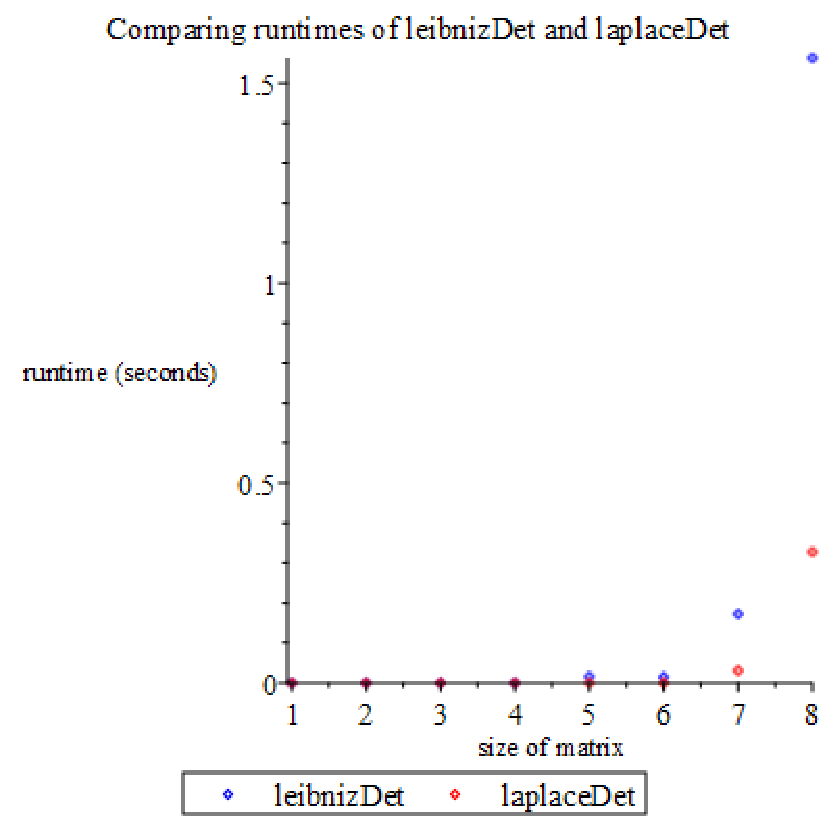
\includegraphics[height=180]{leibniz-laplace}
    \end{center}

    Runtimes are similar --- both run in exponential time.

\end{frame}

\begin{frame}{Laplace expansion vs LU decomposition}

    \begin{center}{}
        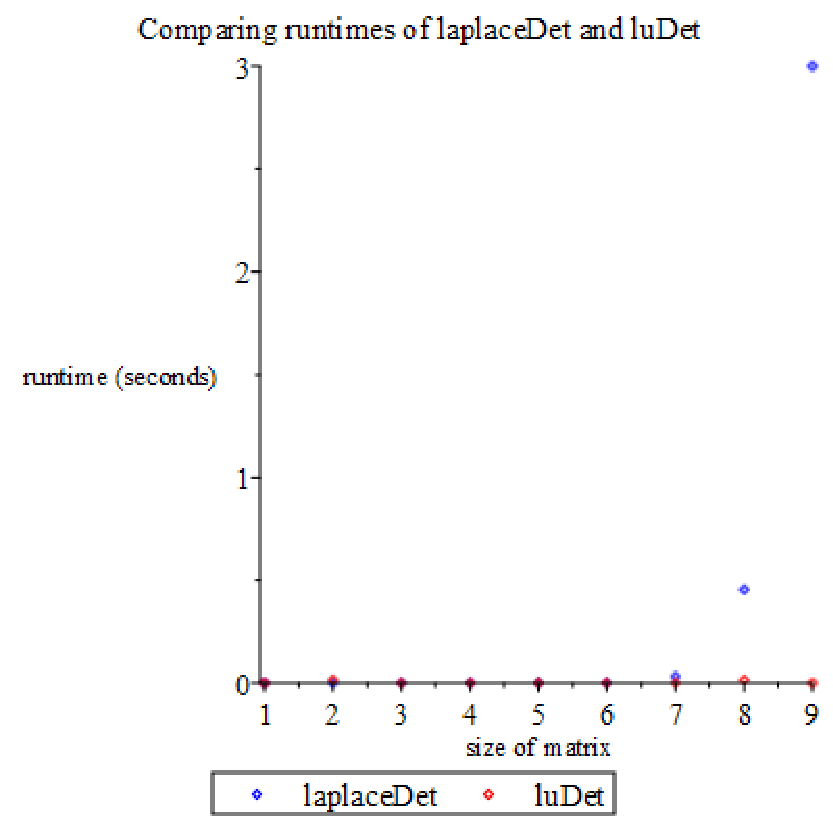
\includegraphics[height=180]{laplace-lu}
    \end{center}

    The difference between the exponential and polynomial-time function is clear.
    % Let's look at a better algorithm.
\end{frame}

\subsection{Gaussian elimination}

\begin{frame}{Gaussian elimination}

    \begin{itemize}

        \item The determinant of a triangular matrix can be computed by taking the product of its
            diagonal entries (which is a quick $\mathcal{O}(n)$ operation).

        \item Any invertible square matrix can be transformed into echelon form by performing
            Gaussian elimination, which takes $\mathcal{O}(n^3)$ time.

    \end{itemize}

    So how does it compare to LU decomposition?

\end{frame}

\begin{frame}{Gaussian elimination vs LU decomposition}

    \begin{center}{}
        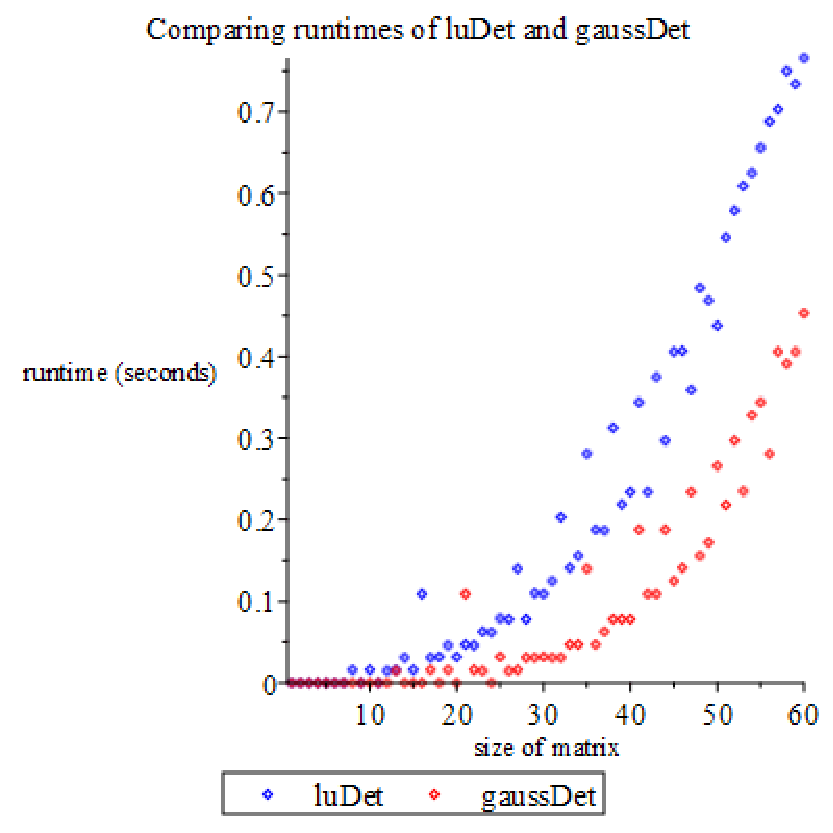
\includegraphics[height=180]{lu-gauss}
    \end{center}

    The difference in runtimes is small (a constant factor).

\end{frame}

\begin{frame}{Gaussian elimination (cont.)}


    Conventional Gaussian elimination requires division.
    This has two problems:
    \begin{itemize}
        \item Over $\mathbb{M}(n; \mathbb{R})$ solutions maybe inexact, so precision is lost.
        \item Division is not a ring operation,
            so would not necessarily work on matrices over a ring.
    \end{itemize}

    This is can be addressed by using\dots

\end{frame}

\subsection{Bareiss algorithm}

\begin{frame}{Bareiss algorithm}

    \begin{itemize}

        \item Addresses the issue of precision-loss by performing \emph{integer-preserving}
            Gaussian elimination on integer matrices.

        \item The runtime complexity is $\mathcal{O}(n^3)$ which is the same as conventional
            Gaussian Elimination, whilst preserving exactness.

            % TODO: possibly give an algorithm?

    \end{itemize}

    % This is very complicated.  Are there any easier exact algorithms that run in polynomial time?

\end{frame}

\subsection{Bird's algorithm}

\begin{frame}{Bird's algorithm}

    Define $\mu : \mathbb{M}(n) \to \mathbb{M}(n)$:
    \[
        \mu(X) =
        \begin{pmatrix}{}
            \mu_{2,2} - x_{2,2} & x_{1,2}             & \cdots & x_{1,n-1}           & x_{1,n} \\
            0                   & \mu_{3,3} - x_{3,3} & \cdots & x_{2,n-1}           & x_{2,n} \\
            \vdots              & \vdots              & \ddots & \vdots              & \vdots \\
            0                   & 0                   & \cdots & \mu_{n,n} - x_{n,n} & x_{n-1,n} \\
            0                   & 0                   & \cdots & 0                   & 0
        \end{pmatrix}
    \]
    and $F_A : \mathbb{M}(n) \to \mathbb{M}(n)$,
    with $A \in \mathbb{M}(n)$
    \begin{align*}{}
        F_A(X)    & = \mu(X)\cdot A \\
        F_A^2(X)  & = \mu(F_A(X)) \cdot A \\
                  & \vdots \\
        F_A^n(X)  & = \mu(F_A^{n-1}(X)) \cdot A \\
    \end{align*}

\end{frame}

\begin{frame}{Bird's algorithm (cont.)}

    \begin{block}{Bird's Theorem}
        \[
            F_A^{n-1}(A) =
            \begin{pmatrix}{}
                d      & 0      & \cdots & 0 \\
                0      & 0      & \cdots & 0 \\
                \vdots & \vdots & \ddots & \vdots \\
                0      & 0      & 0      & 0
            \end{pmatrix}
            \text{with} \ d =
            \begin{cases}{}
                \det(A)  & \text{odd} \ n \\
                -\det(A) & \text{even} \ n \\
            \end{cases}
        \]
    \end{block}

    \begin{itemize}

        \item Enables the \emph{division-free} computation of determinants in
            $\mathcal{O}(n\cdot M(n))$ where $M(n)$ is the runtime complexity of the matrix
            multiplication algorithm used.

        \item If the conventional $\mathcal{O}(n^3)$ matrix multiplication algorithm is used,
            then Bird's algorithm will run in $\mathcal{O}(n^4)$ time.

        \item But this can be reduced to $\mathcal{O}(n^{3.8})$ by using the
            \emph{Strassen algorithm} for matrix multiplication.

    \end{itemize}

\end{frame}

\begin{frame}{Bird's algorithm vs LU decomposition}

    \begin{center}{}
        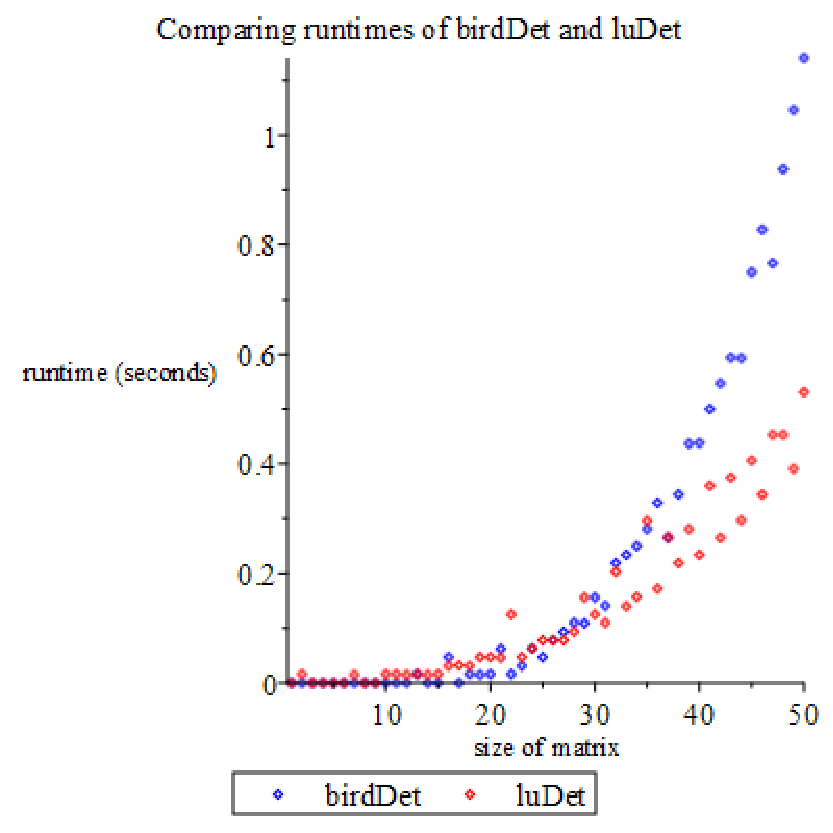
\includegraphics[height=180]{bird-lu}
    \end{center}

    Bird's runtimes increase noticeably more rapidly than LU decomposition,
    but it's still polynomial.

\end{frame}

\section{Epilogue}

\subsection{Summary of determinant algorithms}

\begin{frame}{Summary of determinant algorithms}

    \begin{center}
        \begin{tabular}{l l l}
            \toprule
            \emph{Algorithm}     & \emph{Runtime}           & \emph{Exact?} \\
            \midrule
            Leibniz formula      & $\mathcal{O}((n+1)!)$    & Yes \\
            Laplace expansion    & $\mathcal{O}(n!)$        & Yes \\
            LU decomposition     & $\mathcal{O}(n^3)$       & No \\
            Gaussian elimination & $\mathcal{O}(n^3)$       & No \\
            Bareiss algorithm    & $\mathcal{O}(n^3)$       & Yes \\
            Bird's algorithm     & $\mathcal{O}(n^{3.8})$   & Yes \\
            \bottomrule
        \end{tabular}
    \end{center}

\end{frame}

\subsection{How fast is Maple's implementation?}

\begin{frame}{How fast is Maple's built-in determinant function?}

    \begin{center}{}
        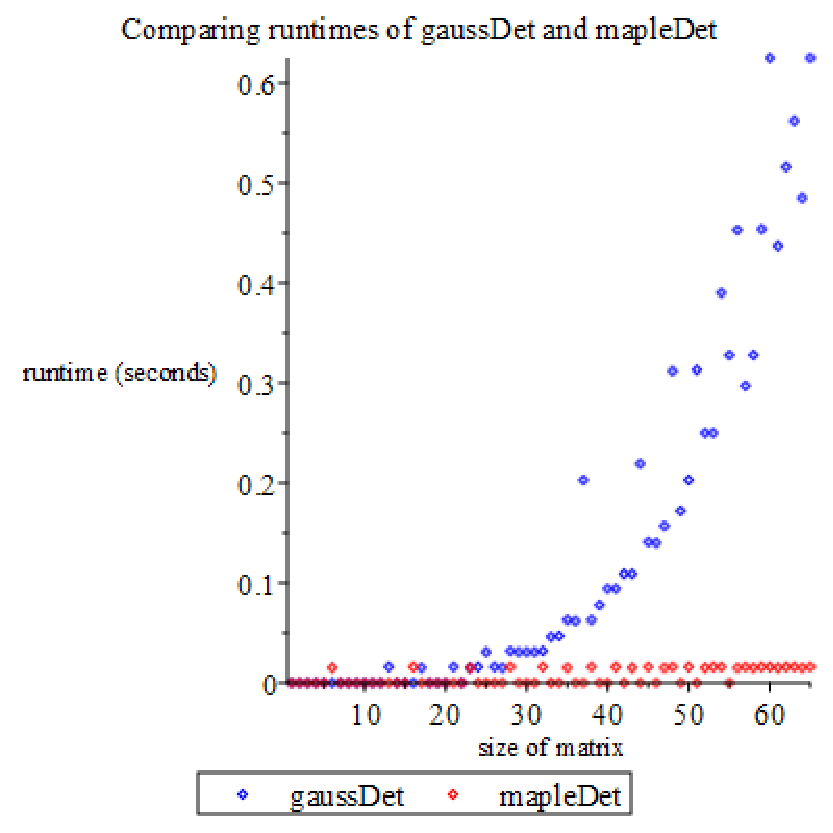
\includegraphics[height=180]{gauss-maple}
    \end{center}

    Very. Maple's optimisation means a fair comparison cannot be made.

\end{frame}

\begin{frame}

    \begin{center}
        \Huge{Thanks!}
    \end{center}

\end{frame}

\end{document}
